\chapter{Результаты}

Мною был написана программа, реализующая имитационную модель сети со следующей топологией:
\begin{itemize}
\item $N=20$ TCP-источников, $N$ TCP-приёмников, двух маршрутизаторов $R1$
  и $R2$ между источниками и приёмниками ($N$ — не менее 20);
\item между TCP-источниками и первым маршрутизатором установлены
  дуплексные соединения с пропускной способностью 100 Мбит/с и
  задержкой 20 мс очередью типа DropTail;
\item между TCP-приёмниками и вторым маршрутизатором установлены
  дуплексные соединения с пропускной способностью 100 Мбит/с и
  задержкой 20 мс очередью типа DropTail;
\item между маршрутизаторами установлено симплексное соединение
  ($R1$--$R2$) с пропускной способностью 20 Мбит/с и задержкой 15 мс
  очередью типа RED, размером буфера 300 пакетов; в обратную сторону~---
  симплексное соединение ($R2$--$R1$) с пропускной способностью 15 Мбит/с и
  задержкой 20 мс очередью типа DropTail;
\item данные передаются по протоколу FTP поверх TCPReno;
\item параметры алгоритма RED: $q_{\min}=75$, $q_{\max}=150$, $q_w=0,002$, $p_{\max}=0.1$;
\item максимальный размер TCP-окна 32; размер передаваемого пакета 500
  байт; время моделирования~--- не менее 20 единиц модельного времени.
\end{itemize}

Полная реализация программы приведена в разделе \textbf{Приложения},
для вывода графиков была использована программа GNUPLOT.

Смоделировав сеть с указанными параметрами и запустив gnuplot-скрипт,
я получил следующий график (рис.~\ref{fig:3.1}).

\begin{figure}[!ht]
  \centering
  \includegraphics[width=0.6\linewidth]{image/queues_75-150_classic.eps}
  \caption{График длины очереди и средней длины очереди на
    линке (R0--R1) ($q_{\min}=75$, $q_{\max}=150$, $q_w=0.002$, $p_{\max}=0.1$,
    TCP типа TCP/Reno)}
  \label{fig:3.1}
\end{figure}

Как мы видим из первого графика, в момент времени $t=1$~c достигается
максимальные длины очереди 140000 пакетов и средней длины очереди
120000 пакетов, а при дальнейшем моделировании длина очереди
варьируются от 0 до 70000 пакетов, а средняя очередь от 0 до 60000,
наступает стационарное состояние.

Для выявления влияния пороговых значений на длину очереди смоделировал
сеть и вывел на одном графике траектории  средней длины очереди при разных
пороговых значениях и при одинаковых остальных параметрах
(рис.~\ref{fig:3.2}).

\begin{figure}[!ht]
  \centering
  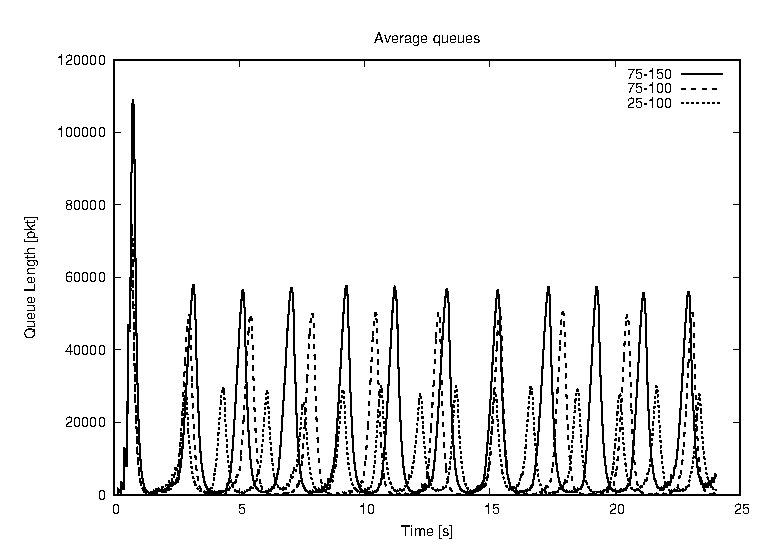
\includegraphics[width=0.6\linewidth]{image/av_queues_maxthresh.eps}
  \caption{График средней длины очереди для разных пороговых значений}
  \label{fig:3.2}
\end{figure}

Как видно из графика, %уменьшение
увеличение диапазона между $q_{\min}$ и $q_{\max}$ способствует
увелечению длины очереди на линке.

Для сравнений различных модификаций смоделировали сеть, задав в
качестве очереди RED, GRED, NLRED,
RARED (рис.~\ref{fig:3.3},~\ref{fig:3.4},~\ref{fig:3.5},~\ref{fig:3.6}).

\begin{figure}[!ht]
  \centering
  \includegraphics[width=0.6\linewidth]{image/av_queues_classic_gentle.eps}
  \caption{Средняя длина очереди RED и GRED при одинаковых условиях}
  \label{fig:3.3}
\end{figure}

\begin{figure}[!ht]
  \centering
  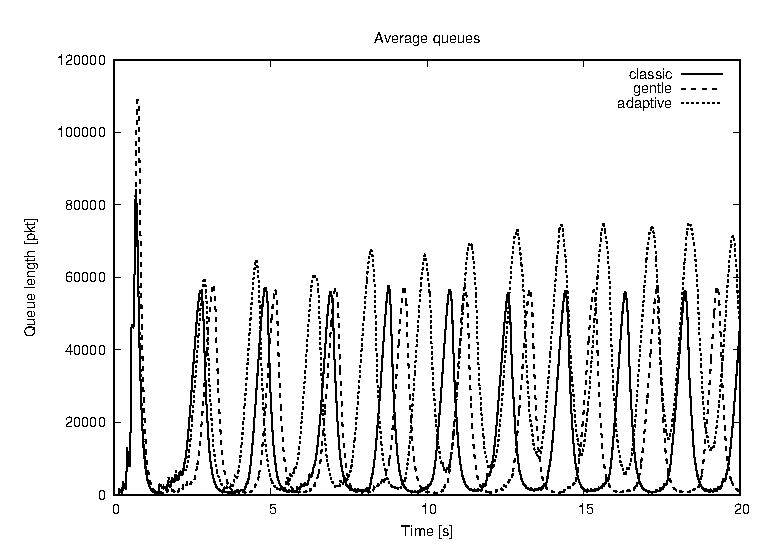
\includegraphics[width=0.6\linewidth]{image/av_queues_3types.eps}
  \caption{Средняя длина очереди RED, GRED, ARED при одинаковых условиях}
  \label{fig:3.4}
\end{figure}

\begin{figure}[!ht]
  \centering
  \includegraphics[width=0.6\linewidth]{image/queues_3types.eps}
  \caption{Длина очереди RED, GRED, ARED при одинаковых условиях}
  \label{fig:3.5}
\end{figure}

\begin{figure}[!ht]
  \centering
  \includegraphics[width=0.6\linewidth]{image/av_queues_classic_nonlinear.eps}
  \caption{Средняя длина очереди RED, NLRED при одинаковых условиях}
  \label{fig:3.6}
\end{figure}

Различие между RARED с остальными модификациями легко объяснить его
автоматическим выбором минимального и максимального пороговых
величин. Средняя очередь при Gentle RED до стационарного состояния
гораздо выше, что обьяснется его более мягким
алгоритмом. Моделирование NLRED не показало никаких различий с
классическим RED, что указывет на неработаспособность патча.

Смоделировали сеть при разных TCP(Reno, Vegas и Newreno)
(рис.~\ref{fig:3.7},~\ref{fig:3.8},~\ref{fig:3.9}).

\begin{figure}[!ht]
  \centering
  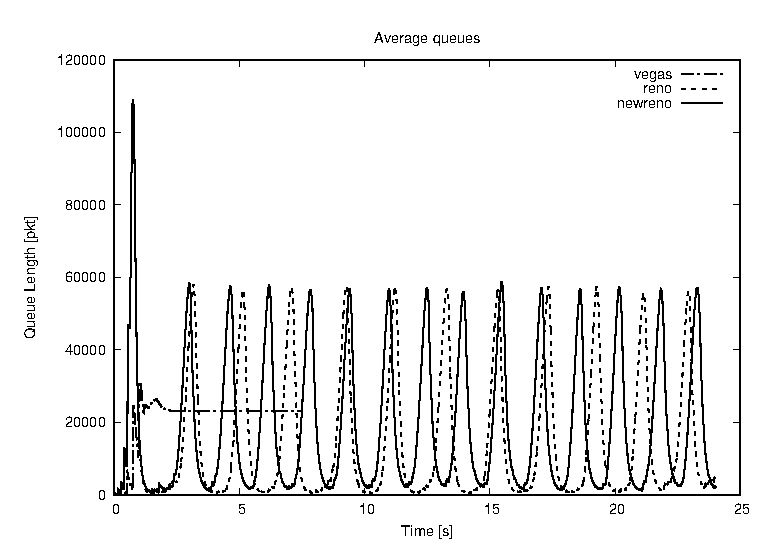
\includegraphics[width=0.6\linewidth]{image/av_queues_tcp.eps}
  \caption{График длины очередей на линке (R0-R1) при разных TCP}
  \label{fig:3.7}
\end{figure}

\begin{figure}[!ht]
  \centering
  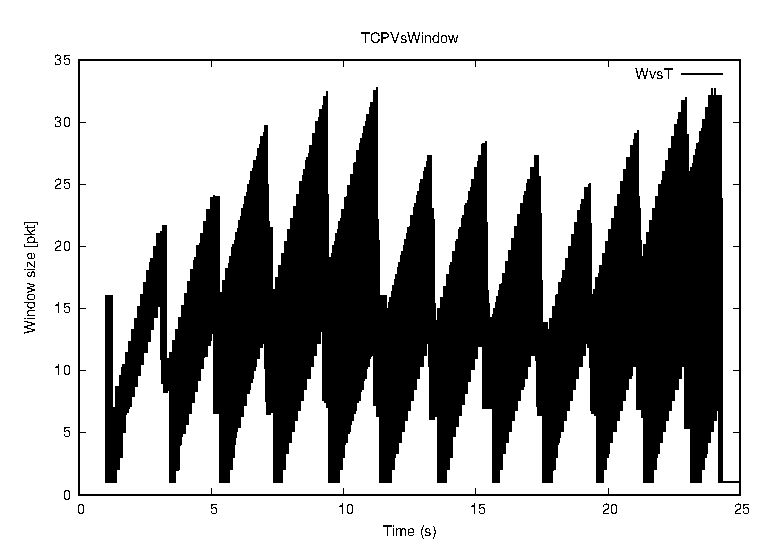
\includegraphics[width=0.6\linewidth]{image/TCP_75-150_classic.eps}
  \caption{График размера TCP-окна для всех источников (TCP типа TCP/Reno)}
  \label{fig:3.8}
\end{figure}

\begin{figure}[!ht]
  \centering
  \includegraphics[width=0.6\linewidth]{image/TCP_vegas.eps}
  \caption{График размера TCP-окна для всех источников (TCP типа TCP/Vegas)}
  \label{fig:3.9}
\end{figure}

Такое заметное отличие TCP/Vegas от TCP/Reno и TCP/Newreno объясняется
тем, что он использует альтернативный подход к управлению
перегрузкой. Вместо использования потери пакетов в качестве индикатора
перегрузки сети он анализирует задержку пакетов в сети и использует
данную информацию для определения, происходит ли перегрузка в сети.




